\documentclass[
12pt,
oneside,
a4paper,
brazil
]{abntex2}

\usepackage{hyperref}
\usepackage[utf8]{inputenc}
\usepackage{mathptmx}
\usepackage[T1]{fontenc}
\usepackage{indentfirst}
\usepackage{enumitem}
\usepackage{setspace}
\usepackage[section]{placeins}
\usepackage{amsmath}
\usepackage{graphicx}
\usepackage{float}

% Informações
\titulo{Análise de Desempenho - Computação Paralela}
\autor{Caio Collino Troiano \\ Thiago Pereira Lins da Silva \\ Vinicius Vianna Egydio de Carvalho}
\local{São Paulo}
\data{2026}

\instituicao{
Centro Universitário Senac
\par
Ciência da Computação
}

\hypersetup{
colorlinks=true,
linkcolor=blue
}

\tipotrabalho{Documento Técnico}
\preambulo{Documento de resultados de pesquisa desenvolvido para a disciplina de Computação Paralela.}

\begin{document}

\imprimircapa

\tableofcontents*
\cleardoublepage

\OnehalfSpacing

\chapter{Resultados e Análise}

\section{Objetivo}

O objetivo deste experimento foi avaliar o desempenho de uma implementação paralela em comparação com sua versão sequencial, analisando o impacto da quantidade de threads no tempo de execução, no speedup e na eficiência do algoritmo.

Os testes foram realizados para diferentes tamanhos de entrada ($N = 1000$, $2000$, $4000$, $8000$ e $10000$), utilizando 2, 4, 8 e 16 threads. Para cada configuração foram obtidos os tempos médios de execução, permitindo o cálculo do speedup e da eficiência.

\section{Resultados Obtidos}

\subsection{Tempo de Execução}

A Figura \ref{fig:tempo_execucao} apresenta a variação do tempo médio de execução da versão paralela em função do número de threads para cada tamanho de entrada analisado.

\begin{figure}[H]
	\centering
	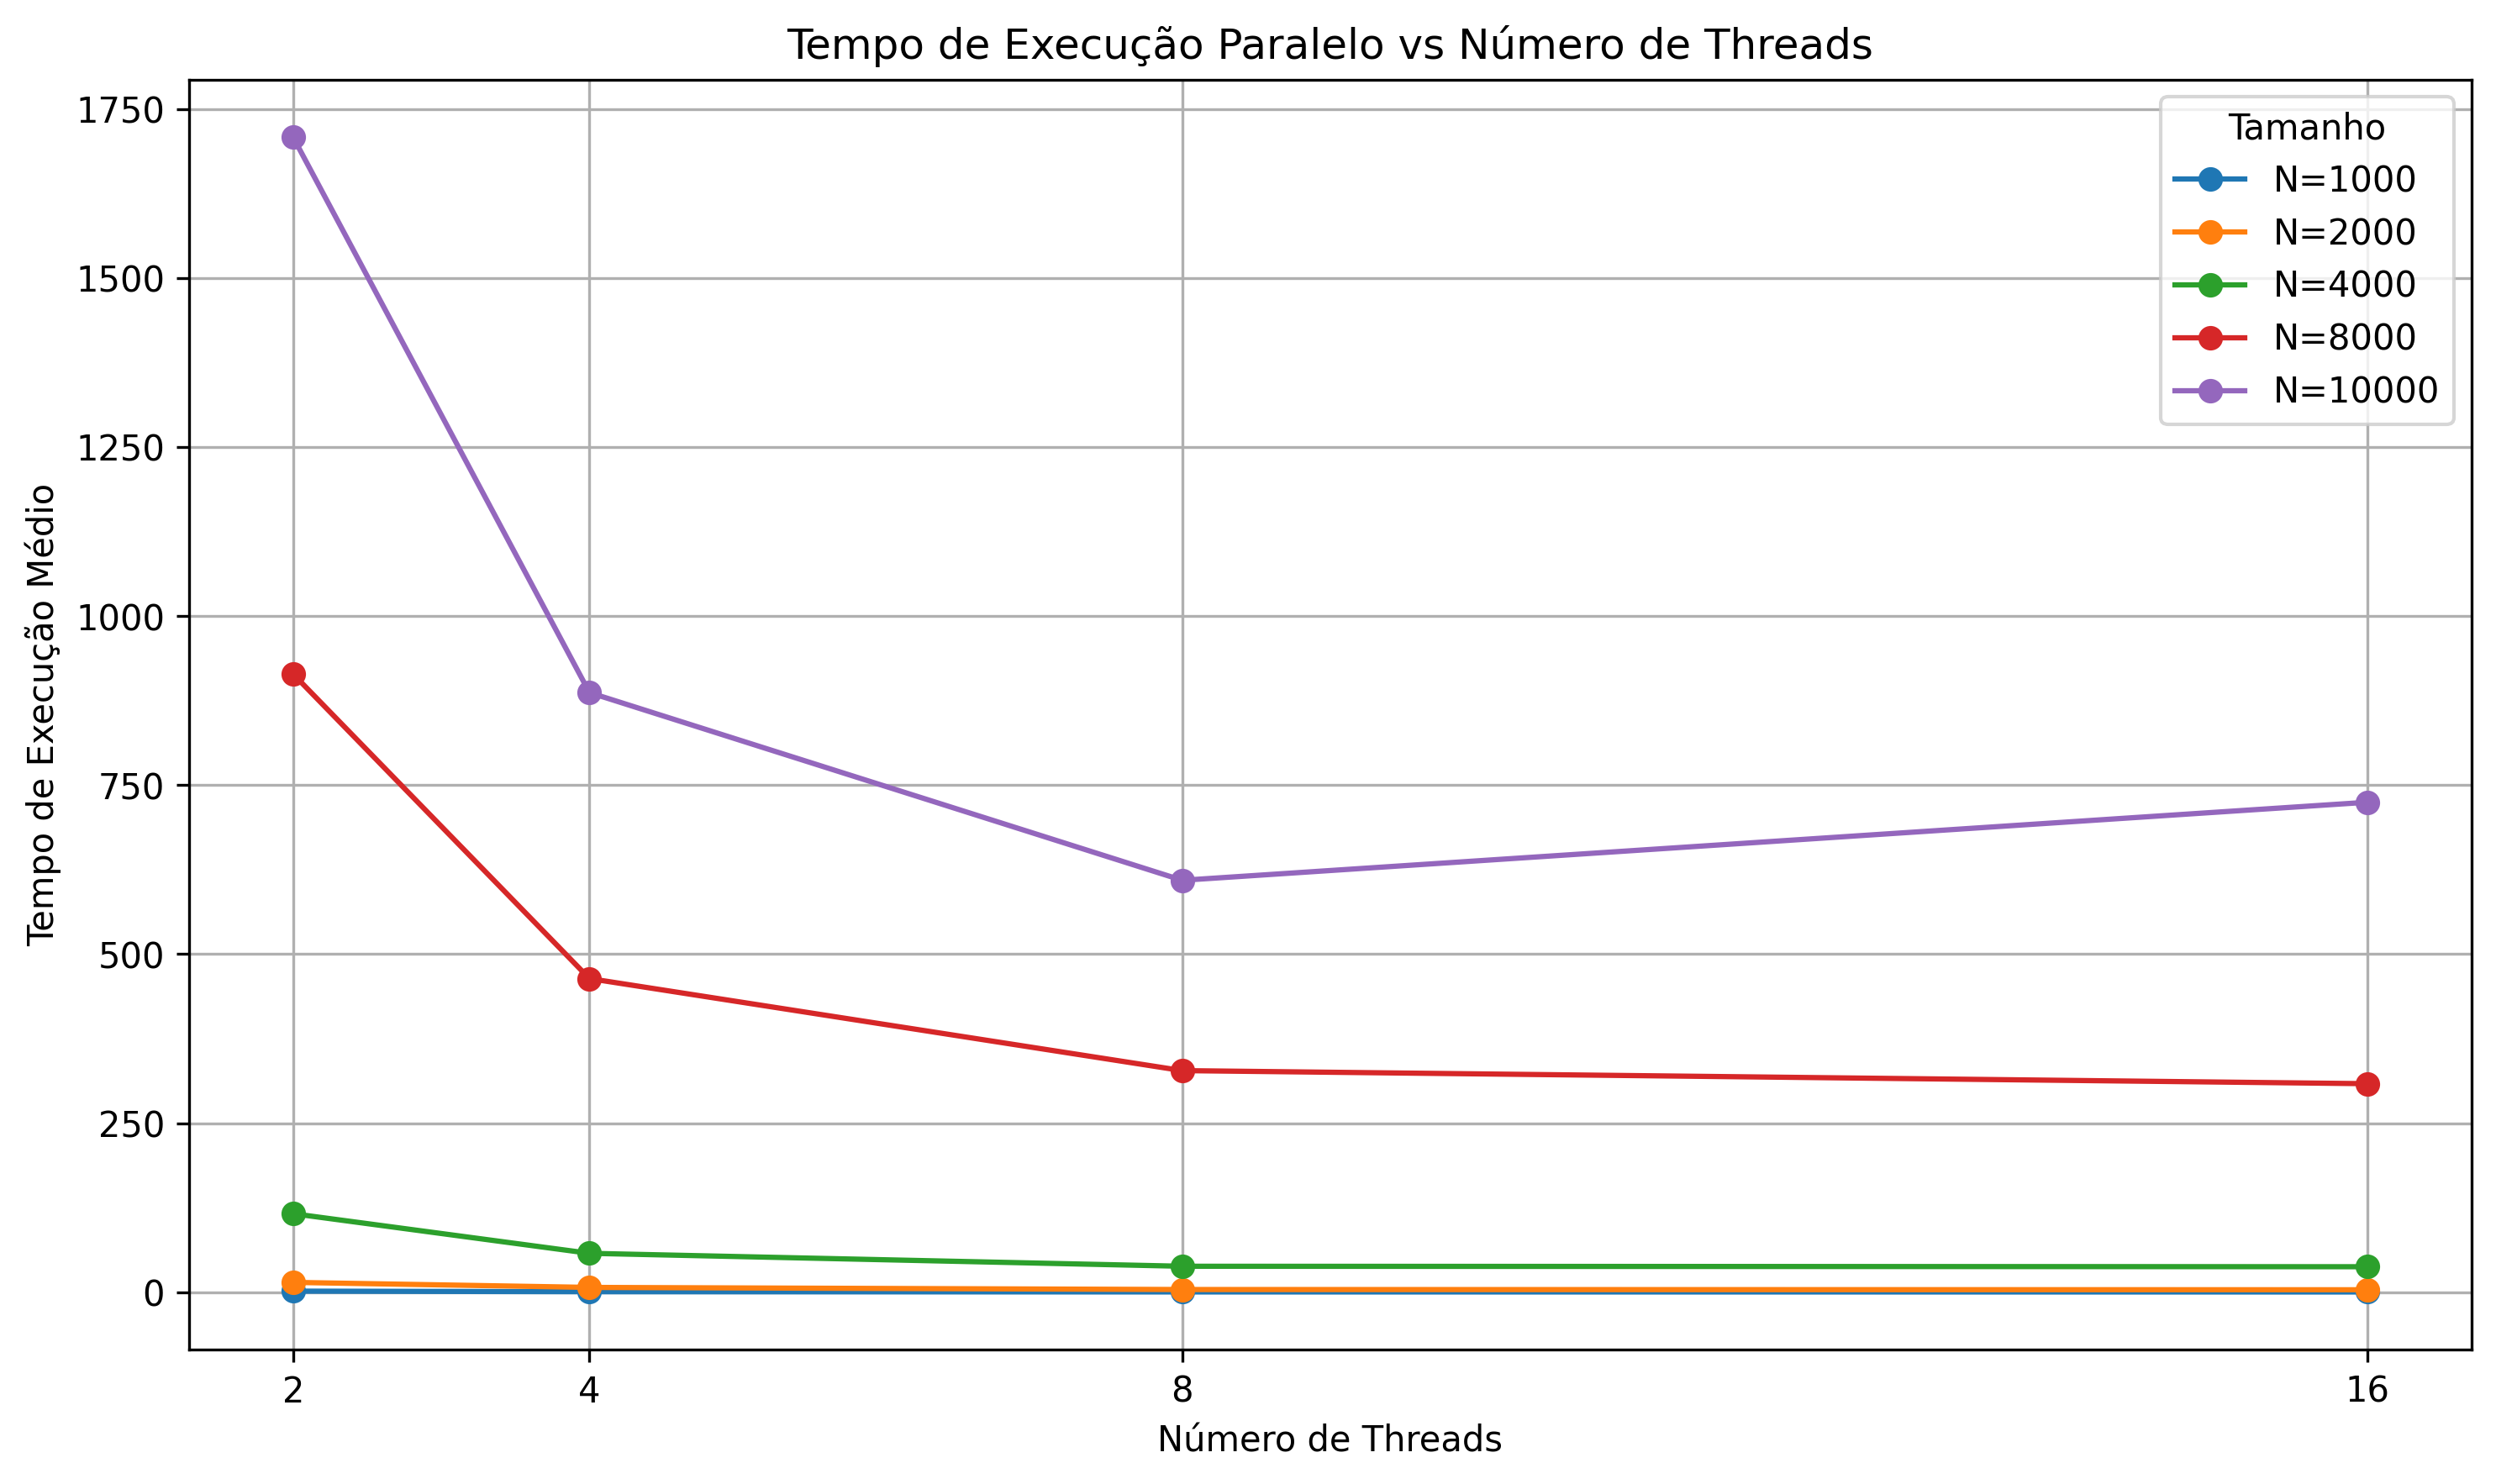
\includegraphics[width=0.85\textwidth]{assets/tempo_execucao_vs_threads.png}
	\caption{Tempo médio de execução em função do número de threads.}
	\label{fig:tempo_execucao}
\end{figure}

Observa-se que o aumento do número de threads reduz significativamente o tempo de execução para todos os tamanhos de entrada. Entretanto, essa redução não ocorre de forma linear, especialmente quando a quantidade de threads ultrapassa oito unidades.

Os maiores ganhos são observados ao passar de 2 para 4 threads e de 4 para 8 threads. A partir desse ponto, os benefícios tornam-se progressivamente menores devido aos custos de sincronização, comunicação e gerenciamento das threads.

\subsection{Speedup}

A Figura \ref{fig:speedup} apresenta o speedup obtido para cada tamanho de entrada em comparação com a execução sequencial.

\begin{figure}[H]
	\centering
	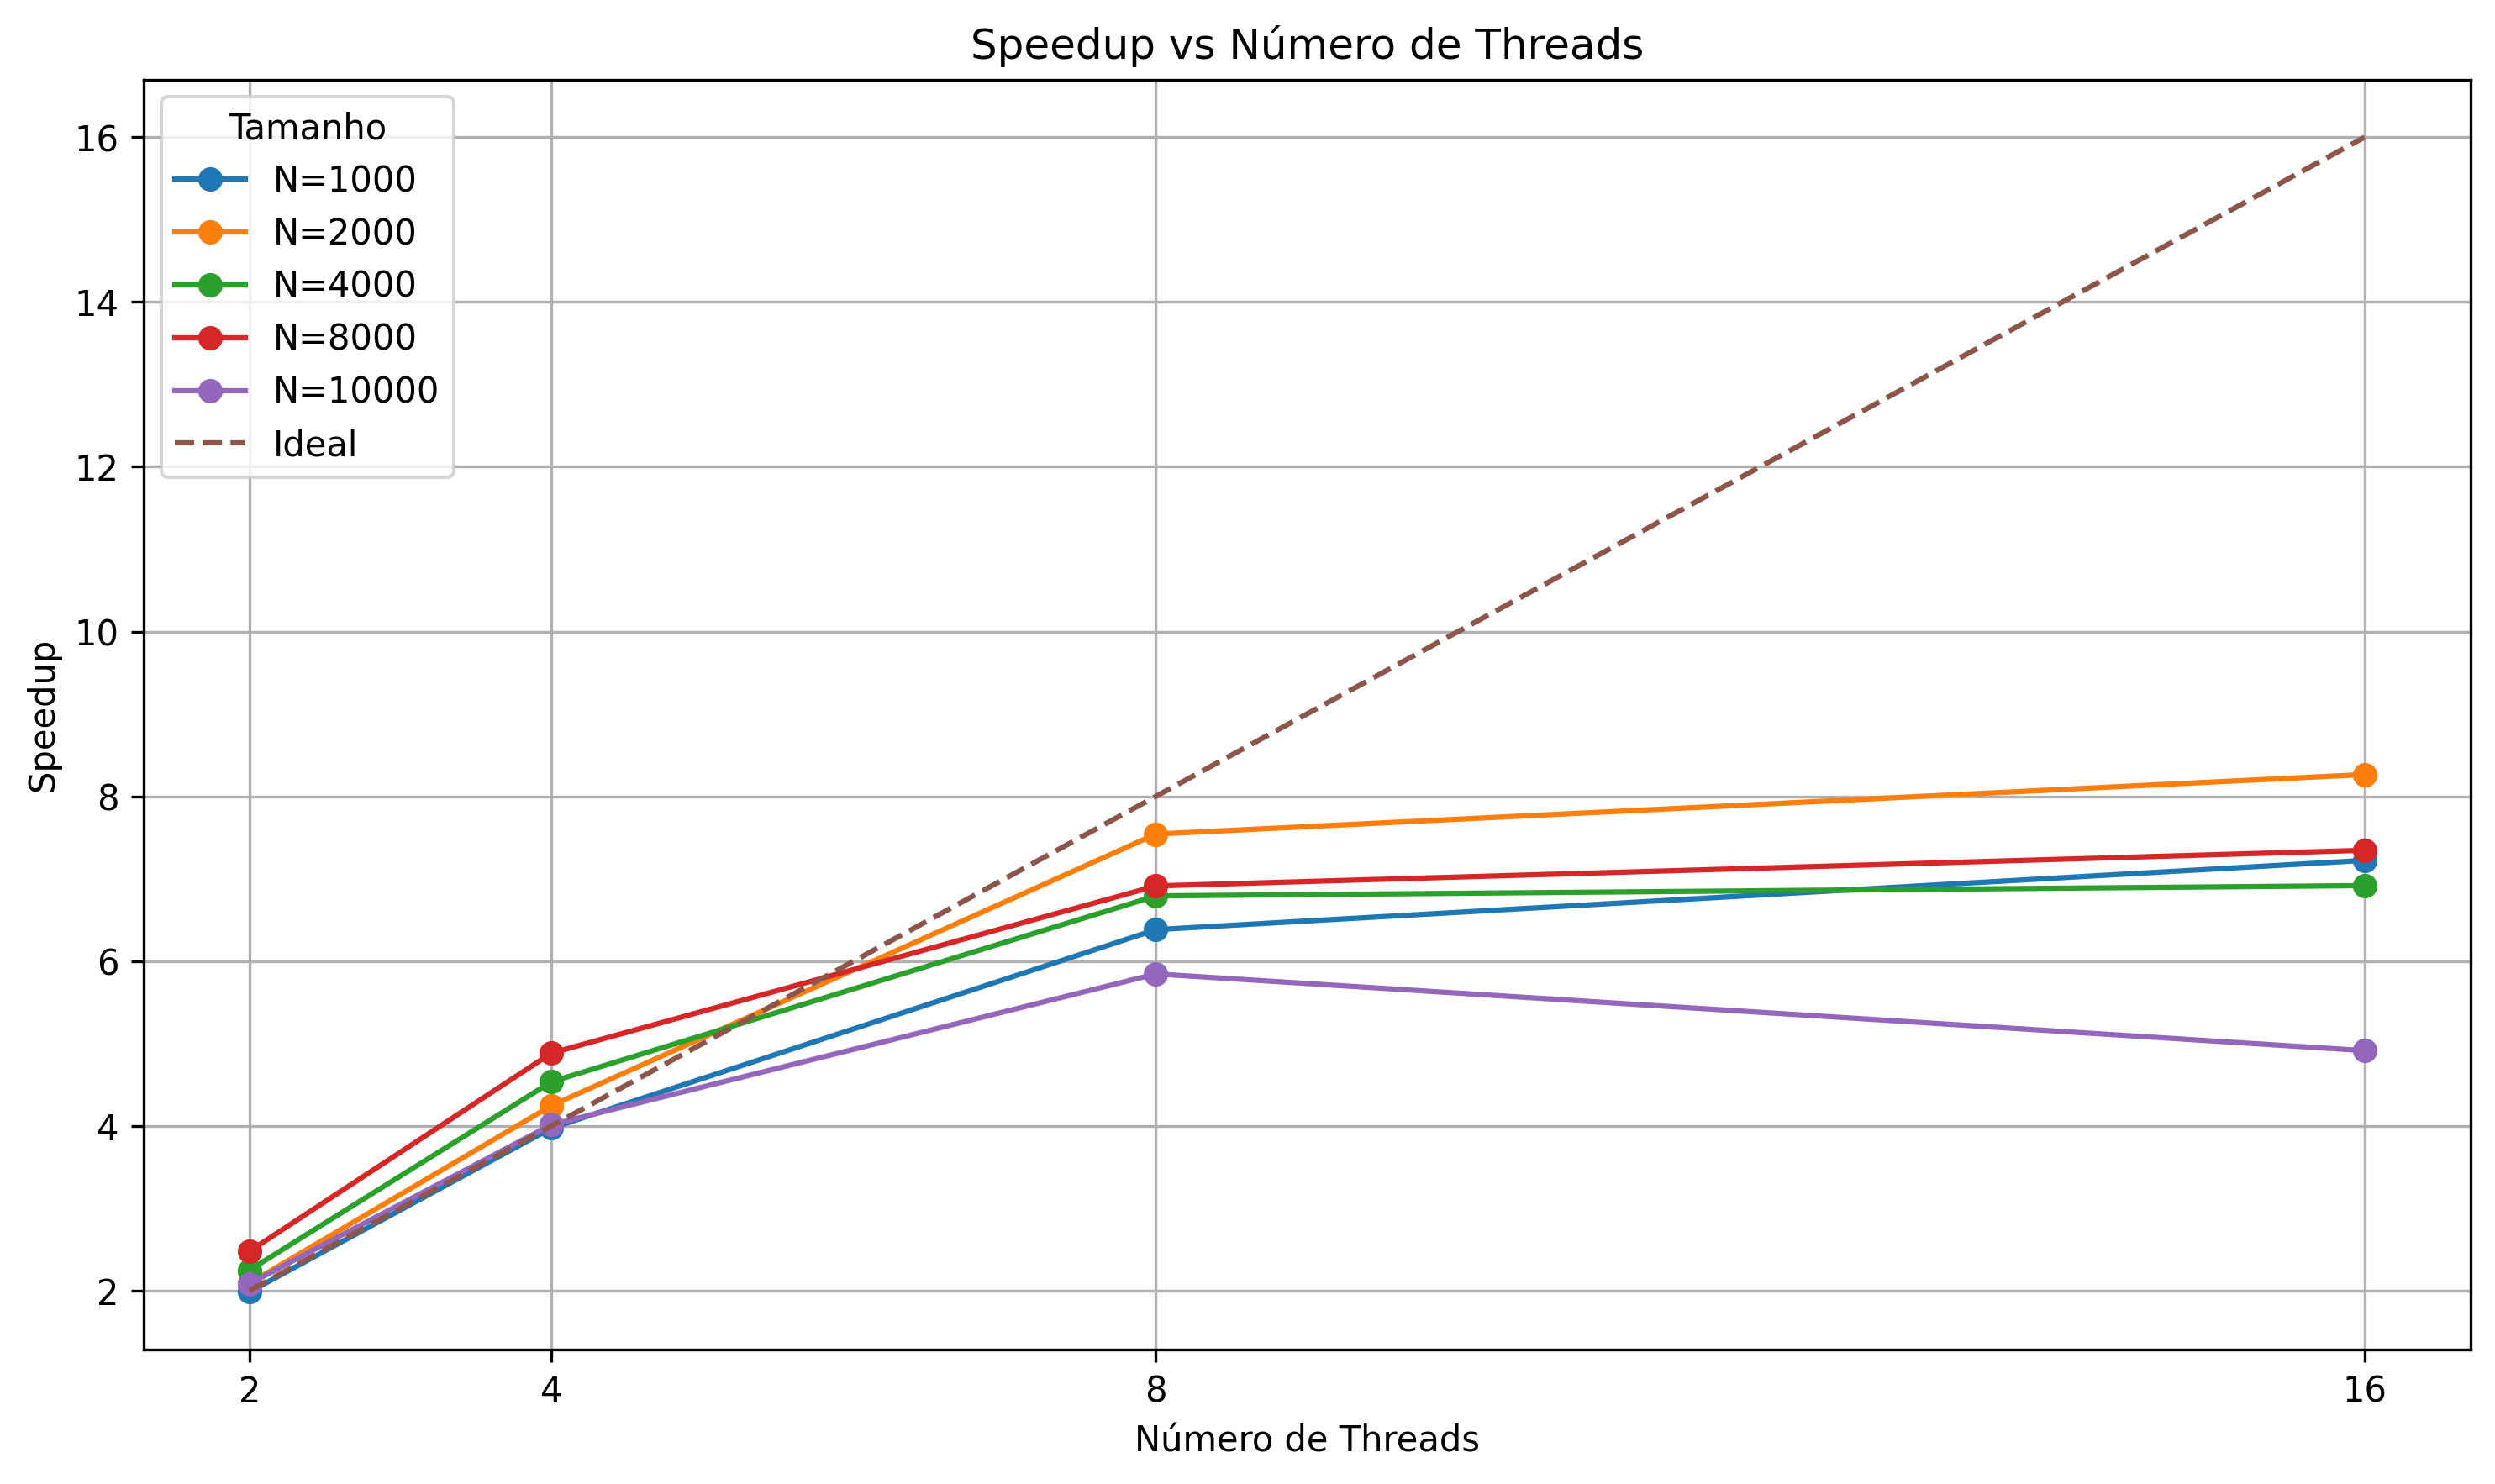
\includegraphics[width=0.85\textwidth]{assets/speedup_vs_threads.png}
	\caption{Speedup em função do número de threads.}
	\label{fig:speedup}
\end{figure}

A linha tracejada presente no gráfico representa o speedup ideal, no qual o ganho de desempenho seria exatamente proporcional ao número de threads utilizadas.

Os resultados mostram que o algoritmo apresenta excelente escalabilidade até aproximadamente 8 threads. Para os tamanhos intermediários ($N = 2000$, $4000$ e $8000$), o speedup obtido aproxima-se significativamente do comportamento ideal.

O melhor resultado foi observado para $N = 2000$ utilizando 16 threads, alcançando um speedup de aproximadamente 8,26 vezes em relação à execução sequencial.

\section{Análise dos Resultados}

Os resultados evidenciam o impacto positivo da paralelização sobre o desempenho do algoritmo.

Para o menor conjunto de dados ($N = 1000$), o speedup cresce rapidamente até 8 threads, alcançando aproximadamente 6,38. Ao utilizar 16 threads, o ganho adicional é pequeno, atingindo cerca de 7,22. Esse comportamento sugere que os custos de gerenciamento das threads passam a representar uma parcela significativa do tempo total de execução.

À medida que o tamanho do problema aumenta, os benefícios da paralelização tornam-se mais evidentes. Para $N = 8000$, por exemplo, o tempo de execução foi reduzido de aproximadamente 2265 unidades de tempo na versão sequencial para cerca de 308 unidades utilizando 16 threads.

Esse comportamento está relacionado ao aumento da granularidade do trabalho. Problemas maiores oferecem mais operações independentes que podem ser distribuídas entre as threads, reduzindo proporcionalmente o impacto das sobrecargas associadas ao paralelismo.

Entretanto, observa-se que os ganhos deixam de crescer proporcionalmente ao número de threads disponíveis. Esse fenômeno está diretamente relacionado aos limites impostos pela Lei de Amdahl, segundo a qual a parcela sequencial do algoritmo passa a dominar a execução conforme o número de processadores aumenta.

\section{Análise de Eficiência}

A eficiência é calculada pela Equação \ref{eq:eficiencia}:
\begin{equation}
	E = \frac{S}{P}
	\label{eq:eficiencia}
\end{equation}

onde:
\begin{itemize}
	\item $E$ representa a eficiência;
	\item $S$ representa o speedup;
	\item $P$ representa o número de threads.
\end{itemize}

Os resultados indicam eficiência próxima de 100% para 2 e 4 threads, demonstrando excelente aproveitamento dos recursos computacionais.

Em alguns casos, foram observadas eficiências ligeiramente superiores a 100%. Esse comportamento pode ocorrer devido a fatores como efeitos de cache, otimizações do compilador, escalonamento do sistema operacional ou pequenas variações experimentais.

Com 8 threads, a eficiência permanece elevada, geralmente acima de 80%, indicando que o algoritmo continua escalando adequadamente.

Já para 16 threads ocorre uma queda significativa da eficiência, variando entre aproximadamente 30% e 52%. Isso demonstra que os custos associados à sincronização e ao compartilhamento de recursos passam a limitar os ganhos obtidos com o aumento do paralelismo.

\section{Escalabilidade}

A análise dos gráficos demonstra que a implementação apresenta boa escalabilidade para problemas de médio e grande porte.

Nos menores tamanhos de entrada, o custo de criação e sincronização das threads reduz a efetividade do paralelismo. Em contrapartida, conforme o tamanho do problema cresce, esses custos tornam-se menos relevantes em relação ao volume total de processamento realizado.

Os resultados obtidos para os conjuntos de dados com $N = 4000$ e $N = 8000$ representam os cenários mais próximos do comportamento ideal, evidenciando que o algoritmo consegue aproveitar de forma eficiente os recursos computacionais disponíveis.

Entretanto, a redução do speedup observada para $N = 10000$ ao passar de 8 para 16 threads sugere a existência de gargalos relacionados à arquitetura de hardware, largura de banda de memória ou contenção entre threads.

\section{Limitações do Experimento}

Algumas limitações devem ser consideradas durante a análise dos resultados:
\begin{itemize}
	\item Não foram consideradas métricas de utilização de CPU, memória ou cache.
	\item O experimento foi limitado a no máximo 16 threads.
	\item Não houve comparação entre diferentes estratégias de paralelização.
	\item Fatores externos, como processos concorrentes do sistema operacional, podem ter influenciado os tempos medidos.
	\item As características específicas do hardware utilizado não foram consideradas na análise quantitativa dos resultados.
\end{itemize}

\section{Conclusão}

Os resultados obtidos demonstram que a paralelização foi altamente eficaz para reduzir o tempo de execução do algoritmo.

Observou-se um crescimento consistente do speedup à medida que o número de threads aumentou, especialmente para problemas de maior dimensão. Os melhores resultados foram alcançados entre 8 e 16 threads, dependendo do tamanho da entrada.

A eficiência manteve-se elevada para até 8 threads, indicando excelente aproveitamento dos recursos disponíveis. Entretanto, a utilização de 16 threads evidenciou limitações inerentes à computação paralela, como custos de sincronização, contenção de recursos e aumento da complexidade de gerenciamento.

Conclui-se que a implementação paralela apresenta boa escalabilidade e oferece ganhos substanciais de desempenho para problemas computacionalmente intensivos. Contudo, existe um ponto de saturação a partir do qual o aumento do número de threads deixa de produzir benefícios proporcionais, reforçando a necessidade de identificar a configuração ótima para cada ambiente de execução.

\end{document}

